\documentclass[12pt,a4paper,notitlepage]{report}
\usepackage{polski}
\usepackage[utf8]{inputenc}
\usepackage[polish]{babel}
\usepackage{url}
\usepackage[pdftex]{graphicx}
\usepackage{sidecap}
\usepackage{verbatim}
\usepackage{array}
\usepackage{amsmath}
\usepackage{enumitem}
\usepackage{fancyhdr}
\usepackage[margin=1.8cm]{geometry}
\usepackage{float}
\usepackage{listings}
\usepackage{color}
\usepackage{wrapfig,booktabs}
\usepackage{caption}
\usepackage{wrapfig}

\newcommand\blfootnote[1]{%
  \begingroup
  \renewcommand\thefootnote{}\footnote{#1}%
  \addtocounter{footnote}{-1}%
  \endgroup
}
%remove section whitespace
\usepackage{titlesec}
\titlespacing\section{0pt}{12pt plus 4pt minus 2pt}{0pt plus 2pt minus 2pt}

\makeatletter
\newcommand*{\toccontents}{\@starttoc{toc}}
\makeatother

\renewcommand\thesection{\arabic{section}}
\newcommand{\HRule}{\rule{\linewidth}{0.5mm}} %Do tytułu

\usepackage{etoolbox} %do bibliografi
\patchcmd{\thebibliography}{\chapter*}{\section*}{}{} %żeby bibliografię nie wrzucało na nową stronę


%Do kodu C++
\usepackage{xcolor} % for setting colors

% set the default code style
\lstset{
    frame=tb, % draw a frame at the top and bottom of the code block
    tabsize=4, % tab space width
    showstringspaces=false, % don't mark spaces in strings
    numbers=left, % display line numbers on the left
    breaklines=true,                % sets automatic line breaking
    commentstyle=\color{green}, % comment color
    keywordstyle=\color{blue}, % keyword color
    stringstyle=\color{red} % string color
}
%End kod

\usepackage{amsmath} % Required for \varPsi below
\usepackage{tikz}
\usepackage{varwidth}
\usetikzlibrary{shapes,arrows}
\usepackage{pgfplots}

\usepackage{xfrac} %do ułamków np.: 1\2

\usepackage{longtable} %Do tabli, mogłem się spodziewać

\begin{document}
\renewcommand{\lstlistingname}{Kod} %Zmiana listing na Kod
\renewcommand\bibname{Literatura} %Zmiana "Bibliografia" na "Literatura"
\renewcommand{\tablename}{Tabela} %Zmiana "Tablica" na "Tabela"
%\renewcommand{\figurename}{Zrzut ekranu} %Zmiana figure na Zrzut ekranu

\begin{titlepage}
\begin{center}

\textsc{\LARGE Politechnika Poznańska}\\[0.8cm]
\textsc{\Large Wydział Elektryczny \\ Informatyka}\\[1cm]


\includegraphics[scale=1]{logopoli}
\vspace{.5cm}\\
\textsc{\large Teoria Informacji i Kodowanie}\\[0.2cm]
\textsc{\normalsize Dokumentacja Projektu}\\[.5cm]


% Author and supervisor
\noindent
\begin{minipage}[t]{0.4\textwidth}
\begin{flushleft} \large
\emph{Autorzy:}\\
Michał \textsc{Majka} \\
Nr albumu: 112679\\
Piotr \textsc{Parysek} \\
Nr albumu: 106100
\end{flushleft}
\end{minipage}%
\begin{minipage}[t]{0.4\textwidth}
\begin{flushright} \large
\emph{Prowadzący:} \\
dr inż. Ewa \textsc{Idzikowska}
\end{flushright}
\end{minipage}

%\bigskip
\vspace{2cm}
% Bottom of the page
{\large \today}
%\global\let\newpagegood\newpage %żeby nie było page break po titilepage
%\global\let\newpage\relax %żeby nie było page break po titilepage

\end{center}
\end{titlepage}

\toccontents

\section{Wstęp}
Zadaniem projektowym była implementacja algorytmu kompresji bezstratnej \newline \emph{\textbf{Run-Length Encoding}} (\textbf{RLE}).

Zadanie zrealizowano w środowisku programistycznym Qt Creator 5.5.1\cite{qt} korzystając z kompilatora GCC 4.9.1\cite{gcc}.\\
Do kontroli wersji oraz plików źródłowych wykorzystano oprogramowanie Git\cite{git}, projekt hostowano w repozytorium GitHub\cite{github}.\\
Dokumentację wykonano w \LaTeX \cite{latex} w programie Texmaker 4.5 \cite{program} oraz w edytorze online: ShareLaTeX\cite{sharelatex}. 

\section{Algorytm}
\subsection{Historia}
\textbf{Run-Length Encodings}, również znane jako \textbf{Golomb Codings}, swoje ,,podwaliny'' powstania wiąże z pracami, XVII-wiecznego francuskiego matematyka \textit{Blaise'a Pascal'a}, związanymi z probabilistyką\cite{book}. Koncepcja kodowania powtarzających się znaków była używana od początków istnienia teorii informacji (Shannon 1949, Laemmel 1951), jednakże metodę oraz sposób kodowania wynalazł i opracował \textit{Solomon Wolf Golomb}\cite{golomb}\cite{book}.

\subsection{Zasada działania}
Algorytm jest relatywnie prosty $\rightarrow$ przedstawia powtarzające się wartości jako dany znak i licznik powtórzeń. Na przykład ciąg znaków:
\[pppppppuuuuuttttt......ppppoooooozzzzznnnnannnnn....pppppplllll\]
Zostaje przedstawiony w postaci ciągu:
\[p7u5t5.6p4o6z5n4an5.4p6l5\]

\begin{table}[H]
\begin{tabular}{l l}
Ciąg znaków & Liczba \\\hline
$pppppppuuuuuttttt......ppppoooooozzzzznnnnannnnn....pppppplllll$& 64\\
$p7u5t5.6p4o6z5n4an5.4p6l5$& 26 \\ \hline
& $\sfrac{26}{64}\approx 0.41$
\end{tabular}
\caption{Przykładowa kompresja znakowa}
\end{table}

\section{Opis implementacji}
%Program wykonano w języku C++ z metodami dostarczonymi z Qt.
\subsection{Kodowanie}
% Define block styles
\tikzstyle{decision} = [diamond, draw, fill=green!20, text width=4.5em, text badly centered, node distance=3cm, inner sep=0pt]
\tikzstyle{block} = [rectangle, draw, fill=blue!20, text centered, rounded corners, minimum height=2.5em, execute at begin node={\begin{varwidth}{15em}}, execute at end node={\end{varwidth}}]
\tikzstyle{line} = [draw, -latex']
\subsubsection{Ustalenie znaku kodowania}    
\begin{figure}[H]
\centering
\begin{tikzpicture}[node distance = 2cm, auto]
    % Place nodes
    \node [block] (init) {Zapisanie do QMap wszystkich możliwych wartości bajtu [256 możliwości], wraz z liczbą wystąpień = 0};
    \node [block, below of=init, node distance=2.5cm] (identify) {Wylicznie wystąpień każdego bajtu i zmiana poszczególnych wartości w QMap};
    \node [block, below of=identify] (evaluate) {Wybierz wartość ,,znaku''};
    \node [block, left of=evaluate, node distance=5cm] (update) {Zmień ,,znak''};
    \node [decision, below of=update] (range) {Czy osiągnięto koniec zakresu?};
    \node [decision, below of=evaluate] (decide) {Czy liczba wystąpień znaku jest równa 0?};
    \node [block, below of=decide, node distance=3cm] (stop) {Zapisz znak w zmiennej SIGN};
    \node [block, below of=range, node distance=4.5cm] (qset) {Stwórz QSet wszyskich wystąpień dwubajtowych w danym pliku};
    \node [block, below of=qset] (choose) {Wybierz wartość dwu Bajtową ,,znaku''};
    \node [decision, below of=choose] (signdecide) {Czy ,,znak'' jest w QSet?};
    \node [block, below of=signdecide, node distance=3cm] (over) {Zapisz znak w zmiennej SIGN16};
    \node [block, right of=signdecide, node distance=5cm] (notyet) {Zmień wartość ,,znaku''};
    \node [block, below of=stop] (end) {Koniec.};
    \node [block, right of=over, node distance=5cm] (theend) {Koniec};
    % Draw edges
    \path [line] (init) -- (identify);
    \path [line] (identify) -- (evaluate);
    \path [line] (evaluate) -- (decide);
    \path [line] (decide) -- node [near start] {Nie} (range);
    \path [line] (range) -- node [near start] {Nie} (update);
    \path [line] (update) |- (evaluate);
    \path [line] (decide) -- node {Tak} (stop);
    \path [line] (range) -- node [near start] {Tak} (qset);
    \path [line] (qset) -- (choose);
    \path [line] (choose) -- (signdecide);
    \path [line] (signdecide) -- node [near start] {Nie} (over);
    \path [line] (signdecide) -- node [near start] {Tak} (notyet);
    \path [line] (notyet) |- (choose);
    \path [line] (stop) -- (end);
    \path [line] (over) -- (theend);
\end{tikzpicture}
\caption{Schemat blokowy wyszukiwania ,,znaku''.}
\end{figure}
Do wyszukania ,,znaków'' wykorzystano kontener \lstinline;QMap<quint, int>;, gdzie zmienna \lstinline;quint8; (\lstinline;unsigned byte;) wskazuje na poszczególne możliwe wartości bajta, a zmienna \lstinline;int; wskazuje ilość wystąpień danego bajta w opracowywanym pliku.
\begin{lstlisting}[language=C++, caption={Deklaracja wraz z inicjalizacją kontenera QMap<quint8, int>}]
QMap<quint8, int> IIMap;
for (quint8 i = 0; i < 255; i++) {
	IIMap.insert(i, 0);
}
\end{lstlisting}

W przypadku zdarzenia, że w pliku występują wszystkie możliwe kombinacje bajta, zamiast jedno bajtowego ,,znaku'' zostaje wprowadzony znak dwu bajtowy:
\begin{lstlisting}[language=C++, caption={Deklaracja dwu bajtowej zmiennej znakowej}]
QPair<quint8, quint8> SIGN16;
\end{lstlisting}

\subsubsection{Kodowanie}
\begin{figure}[H]
\centering
\begin{tikzpicture}[node distance = 2cm,auto]
    % Place nodes
    \node [block] (start) {Dopisz do tablicy pliku wyjściowego rozmiar ,,znaku'' oraz bajt/y ,,znak/u''};
    \node [block, below of=start] (jeden) {Wczytaj kolejny bajt};
    \node [decision, below of=jeden] (decyzja) {Czy bajt różni się od poprzedniego?};
    \node [block, right of=decyzja, node distance=5cm] (dwa) {Dopisz Bajt\\ do Listy Elementów};
    \node [block, left of=decyzja, node distance=5cm] (trzy) {Zinkrementuj liczbę\\ wystąpień ostatniego\\ elementu listy};
    \node [block, below of=decyzja, node distance=3.5cm] (cztery) {Zapisz Listę Elementów do Tablicy bajtów wyjściowych};
    \node [block, below of=cztery] (piec) {Zapisz tablicę do pliku};
	\node [block, below of=piec] (szesc) {Koniec.};    
    
    % Draw edges
    \path [line] (start) -- (jeden);
    \path [line] (jeden) -- (decyzja);
    \path [line] (decyzja) -- node [near start] {Tak} (dwa);
    \path [line] (decyzja) -- node [near start] {Nie} (trzy);
    \path [line] (decyzja) -- node [near start] {Koniec tablicy} (cztery);
    \path [line] (dwa) |- (jeden);
    \path [line] (trzy) |- (jeden);
    \path [line] (cztery) -- (piec);
    \path [line] (piec) -- (szesc);        
\end{tikzpicture}
\caption{Schemat blokowy kodowania pliku.}
\end{figure}

Do sprawnego wczytania, zliczenia i zakodowania poszczególnych bajtów stworzono kontener \lstinline;QList; struktury \lstinline;Element;. Struktura \lstinline;Element; posiada dwa pola: \lstinline;quint8 item; $\rightarrow$ oznaczające dany bajt oraz \lstinline;quint32 value; $\rightarrow$ oznaczające ilość wystąpień (Założono, że dany bajt nie powtórzy się więcej jak $4 294 967 295$ razy).
\begin{lstlisting}[language=C++, caption={Główne struktury danych kodowania}]
struct Element {
	quint8 item;
	quint32 value;
};
QList<Element> Elements;
quint8 CurrentByte;
\end{lstlisting}

Zapisanie danych do pliku odbywa się za pośrednictwem tablicy bajtów \lstinline;QByteArray;. Analiza zapisanych znaków odbywa się poprzez przejście przez wcześniej wspomnianą listę: \lstinline;QList<Element>; i odpowiednią interpretację  wartości wystąpień danego znaku. 

Jeżeli wartość powtórzenia danego znaku nie jest większa niż minimalna długość jego zastąpienia, który ma postać ,,znak'' inicjujący, bajt powtarzany, ilość powtórzeń, to wpisywana jest ,,pierwotna postać''.

W przypadku, gdy wartość ilości powtórzeń bajtu jest większa niż maksymalna wartość jaką może osiągnąć bajt - 255 - to postać zastąpienia przybiera postać: czterech bajtów ,,znaku'', bajt powtarzany i cztery bajty licznika.
\begin{lstlisting}[language=C++, caption={Zapisanie i zakodowania danych skompresowanych do pliku}]
if (e.value < 256) {
	OutByteArray.append(SIGN);
	OutByteArray.append(e.item);
	OutByteArray.append(e.value);
} else {
	OutByteArray.append(SIGN);
    OutByteArray.append(SIGN);
    OutByteArray.append(SIGN);
    OutByteArray.append(SIGN);
    OutByteArray.append(e.item);
    QByteArray TempArray;
    TempArray = RLE::IntToHex(e.value);
    OutByteArray.append(TempArray);
}
\end{lstlisting}

\subsection{Dekodowanie}
\begin{figure}[H]
\centering
\begin{tikzpicture}[node distance = 2cm,auto]
    % Place nodes
    \node [block] (start) {Wczytaj rozmiar ,,znaku''};
    \node [block, below of=start] (zero) {Wczytaj ,,znak''};
    \node [block, below of=zero] (jeden) {Wczytaj bajt};
    \node [decision, below of=jeden] (decyzja) {Czy bajt jest rónwy ,,znakowi''?};
    \node [block, right of=decyzja, node distance=5cm] (dwa) {Dopisz Bajt do\\ tablicy bajtów wyjściowych};
    \node [block, left of=decyzja, node distance=5cm] (trzy) {Wczytaj kolejny bajt\\ -powtarzany bajt-\\ i następny bajt -licznik\\ powtórzenia. Dopisz do\\ tablicy bajtów wyjściowych\\ powtarzany bajt w ilości\\ licznika powtórzenia.};
    \node [block, below of=decyzja, node distance=3cm] (cztery) {Zapisz tablicę do pliku};
    \node [block, below of=cztery] (piec) {Koniec.};
    
    % Draw edges
    \path [line] (start) -- (zero);
    \path [line] (zero) -- (jeden);
    \path [line] (jeden) -- (decyzja);
    \path [line] (decyzja) -- node [near start] {Nie} (dwa);
    \path [line] (decyzja) -- node [near start] {Tak} (trzy);
    \path [line] (decyzja) -- node [near start] {Koniec tablicy} (cztery);
    \path [line] (dwa) |- (jeden);
    \path [line] (trzy) |- (jeden);
    \path [line] (cztery) -- (piec);      
\end{tikzpicture}
\caption{Schemat blokowy dekodowania pliku.}
\end{figure}
Dekodowanie odbywa się z pomocą analogicznych struktur / zasad / metod co zostały użyte podczas kodowania.\\[2cm]
W celu ułatwienia kontroli nad plikami po kodowaniu mają one dodawany przyrostek \lstinline;.rlemama;, a podczas dekodowania dodawany przed znacznikiem formatu pliku przyrostek \lstinline;_2;
\newpage
\section{Użytkowanie programu}
Ikony umieszczone w programie zostały pobrane z strony: \url{http://www.flaticon.com/}\cite{ikony}.
\renewcommand{\figurename}{Zrzut ekranu} %Zmiana figure na Zrzut ekranu
\begin{figure}[H]
	\setcounter{figure}{0} %Resetownie licznika
	\centering
	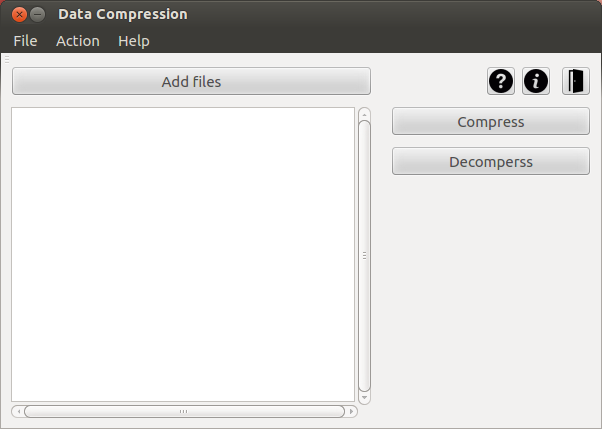
\includegraphics[scale=.7]{start}
	\caption{Wygląd po ,,starcie'' programu.}
\end{figure}
\begin{figure}[H]
	\centering
	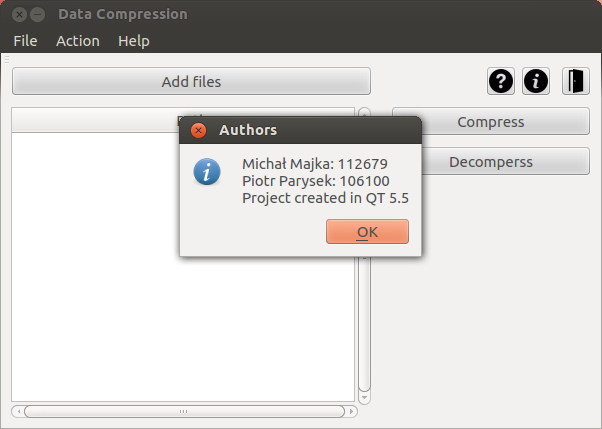
\includegraphics[scale=.7]{info}
	\caption{Włączenie informacji o autorach projektu.}
\end{figure}
\begin{figure}[H]
	\centering
	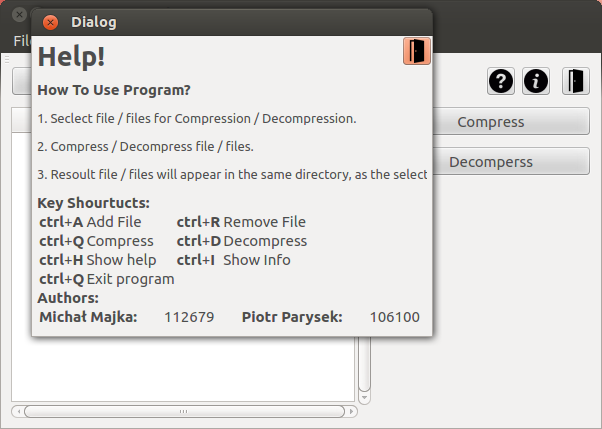
\includegraphics[scale=.7]{help}
	\caption{Włączenie okna pomocy.}
\end{figure}
\begin{figure}[H]
	\centering
	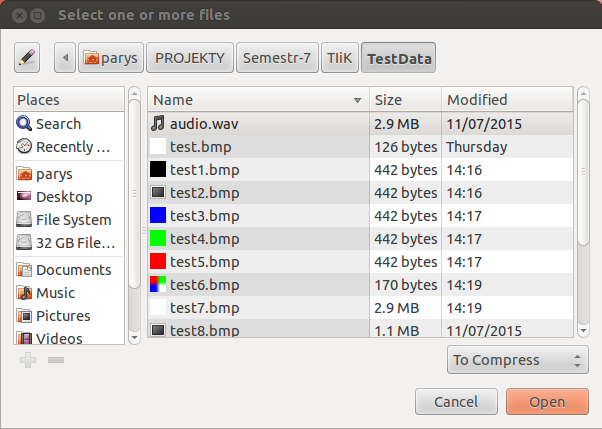
\includegraphics[scale=.7]{take}
	\caption{Przestawienie okna dialogowego wyboru plików, które program może skompresować.}
\end{figure}
\begin{figure}[H]
	\centering
	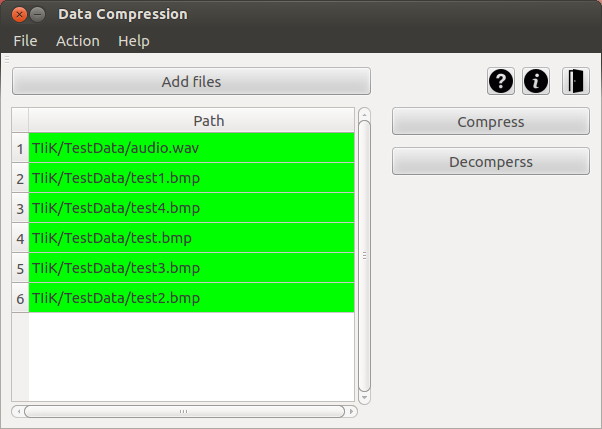
\includegraphics[scale=.7]{com}
	\caption{Przedstawienie plików gotowych do kompresji.}
\end{figure}
\begin{figure}[H]
	\centering
	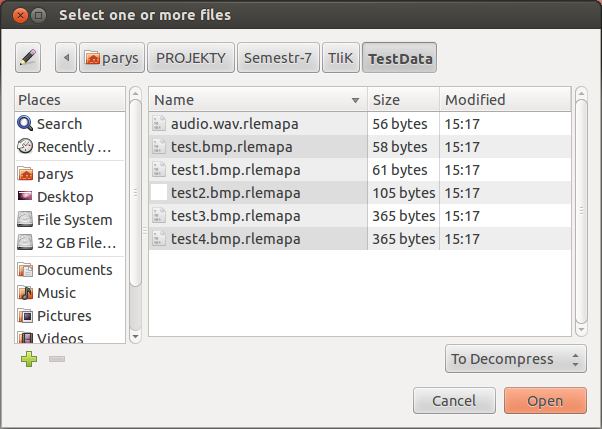
\includegraphics[scale=.7]{take2}
	\caption{Przestawienie okna dialogowego wyboru plików, które program może zdekompresować.}
\end{figure}
\begin{figure}[H]
	\centering
	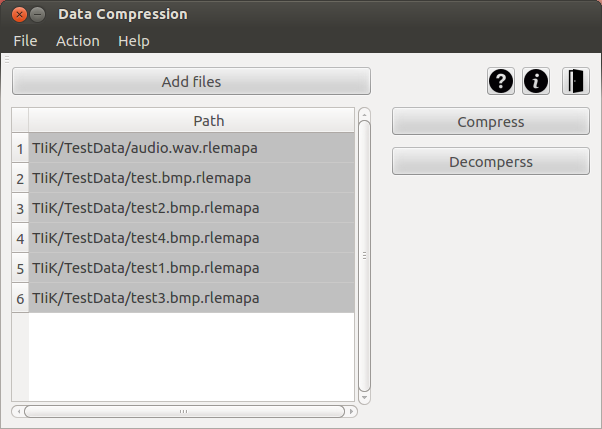
\includegraphics[scale=.7]{decom}
	\caption{Przedstawienie plików gotowych do dekompresji.}
\end{figure}
\begin{figure}[H]
	\centering
	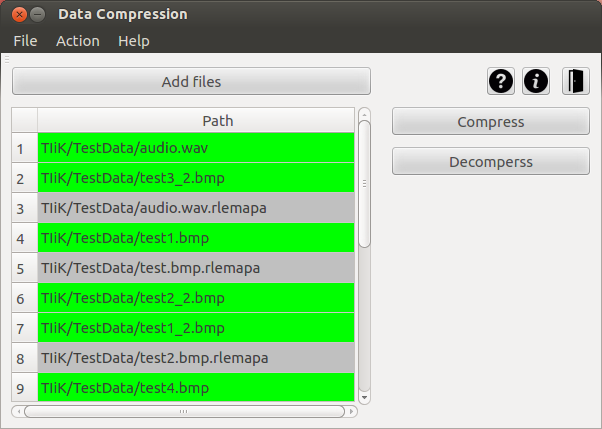
\includegraphics[scale=.7]{all}
	\caption{Przedstawienie plików zdekompresowanych i nie skompresowanych}
\end{figure}

\begin{figure}[H]
	\caption{Przedstawienie komunikatów błędów, gdy nakażemy zdekompresować / skompresować pliki ,,przemieszne''.}
	\centering
	\begin{minipage}{0.45\textwidth}
		\centering
		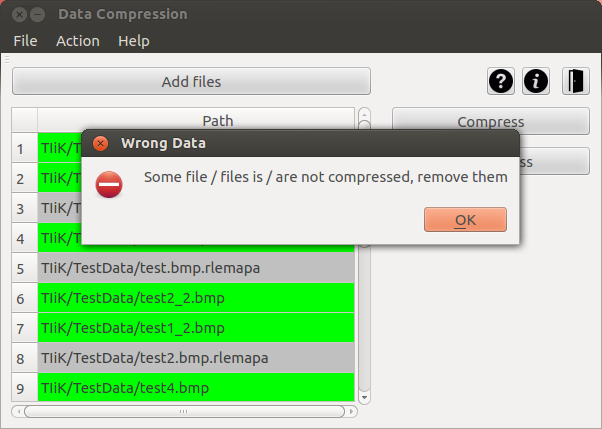
\includegraphics[scale=.4]{error1}
	\end{minipage}\hfill
	\begin{minipage}{0.45\textwidth}
		\centering
		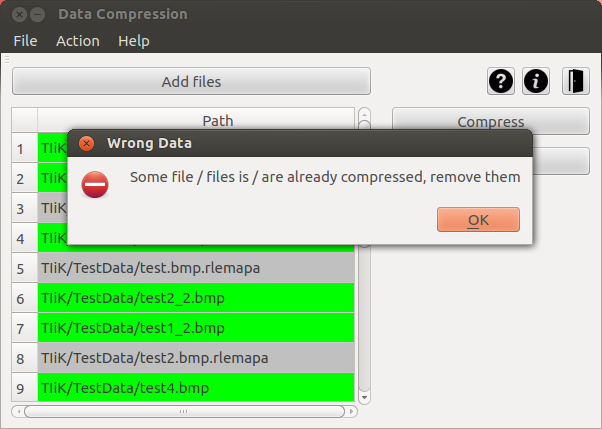
\includegraphics[scale=.4]{error2}
	\end{minipage}
\end{figure}


\begin{figure}[H]
	\centering
	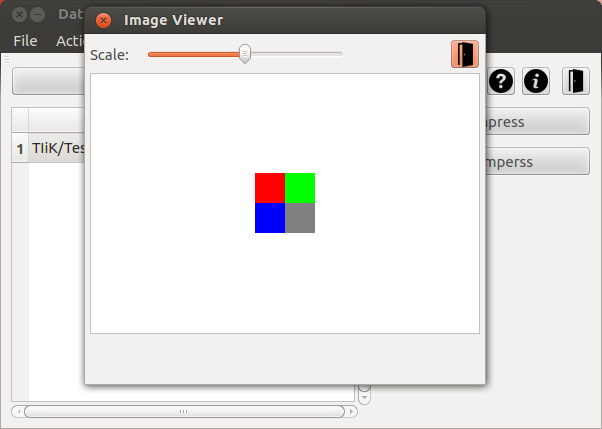
\includegraphics[scale=.7]{imageview_1}
	\caption{Przedstawienie plików zdekompresowanych i nie skompresowanych}
\end{figure}
\begin{figure}[H]
	\centering
	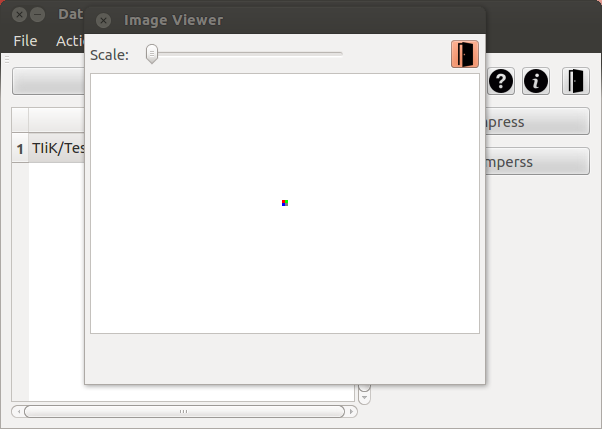
\includegraphics[scale=.7]{imageview_2}
	\caption{Przedstawienie plików zdekompresowanych i nie skompresowanych}
\end{figure}
\begin{figure}[H]
	\centering
	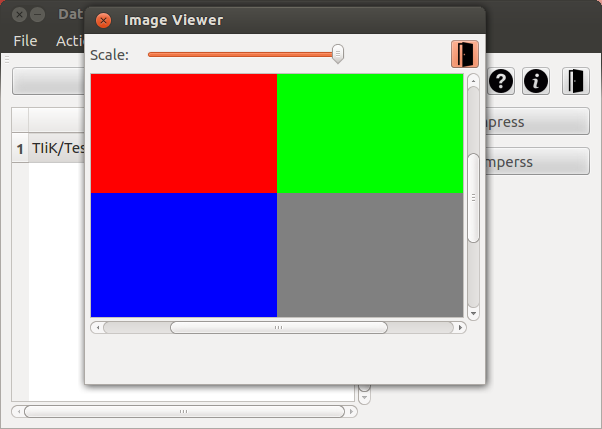
\includegraphics[scale=.7]{imageview_3}
	\caption{Przedstawienie plików zdekompresowanych i nie skompresowanych}
\end{figure}




\section{Testy}
W celu przeprowadzenia testów wykonano kilka prostych obrazków formatu \lstinline;bmp; oraz pobrano z Internetu inne, większe i  bardziej skomplikowane obrazki. Dodatkowo do badań pobrano kilka plików dźwiękowych formatu \lstinline;wav; z strony \url{http://download.wavetlan.com/SVV/Media/HTTP/http-wav.htm}\cite{nuty}.
\begin{table}[H]
\caption{Przykładowe pliki graficzne (powiększone):}
\centering
\begin{tabular}{l l l l l l}
\fbox{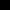
\includegraphics[scale=4]{test1}} & \fbox{
\includegraphics[scale=4]{test2}} & \fbox{
\includegraphics[scale=4]{test3}} & \fbox{
\includegraphics[scale=4]{test4}}
& \fbox{
\includegraphics[scale=4]{test5}} & \fbox{
\includegraphics[scale=10]{test6}}
\end{tabular}
\end{table}

\begin{minipage}{.48\textwidth}
\begin{lstlisting}[language=bash,caption={Przedstawienie plików przed kompresją.}]
ROZMIAR		NAZWA
316002		audio2.wav
869028		audio3.wav
261262		audio4.wav
3009870		audio.wav
8533723		highway.wav
309464		test10.bmp
16000138	test11.bmp
131554		test12.bmp
693122		test13.bmp
442			test1.bmp
442			test2.bmp
442			test3.bmp
442			test4.bmp
442			test5.bmp
170			test6.bmp
3000122		test7.bmp
1163198		test8.bmp
44264		test9.bmp
126			test.bmp
\end{lstlisting}
\end{minipage}
\hfill
\begin{minipage}{.48\textwidth}
\begin{lstlisting}[language=bash,caption={Przedstawienie plików po kompresji.}]
ROZMIAR		NAZWA
315928		audio2.wav.rlemapa
856106		audio3.wav.rlemapa
261239		audio4.wav.rlemapa
56			audio.wav.rlemapa
8447839		highway.wav.rlemapa
85103		test10.bmp.rlemapa
8440758		test11.bmp.rlemapa
76746		test12.bmp.rlemapa
345212		test13.bmp.rlemapa
61			test1.bmp.rlemapa
105			test2.bmp.rlemapa
365			test3.bmp.rlemapa
365			test4.bmp.rlemapa
364			test5.bmp.rlemapa
95			test6.bmp.rlemapa
65			test7.bmp.rlemapa
1163182		test8.bmp.rlemapa
5689		test9.bmp.rlemapa
58			test.bmp.rlemapa
\end{lstlisting}
\end{minipage}


\begin{minipage}{.48\textwidth}
\begin{lstlisting}[language=bash,caption={Przedstawienie plików przed kompresją.}]
ROZMIAR		NAZWA
316002		audio2.wav
869028		audio3.wav
261262		audio4.wav
3009870		audio.wav
8533723		highway.wav
309464		test10.bmp
16000138	test11.bmp
131554		test12.bmp
693122		test13.bmp
442			test1.bmp
442			test2.bmp
442			test3.bmp
442			test4.bmp
442			test5.bmp
170			test6.bmp
3000122		test7.bmp
1163198		test8.bmp
44264		test9.bmp
126			test.bmp
\end{lstlisting}
\end{minipage}
\hfill
\begin{minipage}{.48\textwidth}
\begin{lstlisting}[language=bash,caption={Przedstawienie plików po dekompresji.}]
ROZMIAR		NAZWA
316001		audio2_2.wav
869034		audio3_2.wav
261262		audio4_2.wav
3009873		audio_2.wav
8533722		highway_2.wav
309464		test10_2.bmp
16000138	test11_2.bmp
131599		test12_2.bmp
693121		test13_2.bmp
445			test1_2.bmp
442			test2_2.bmp
442			test3_2.bmp
442			test4_2.bmp
442			test5_2.bmp
170			test6_2.bmp
3000125		test7_2.bmp
1163198		test8_2.bmp
44270		test9_2.bmp
126			test_2.bmp
\end{lstlisting}
\end{minipage}

\subsection{Przedstawienie wyników:}
\begin{comment}
%Zostawię to na cześć swej hańby
\begin{tikzpicture}
\begin{axis}[
    width  = 17cm,
	height = 8cm,
    every axis plot post/.style={/pgf/number format/fixed},
    ybar=5pt,
    bar width=5pt,
    %x=3cm,
    ymin=0,
    axis on top,
    ymax=1000,
    xtick=data,
    enlarge x limits=0.2,
    symbolic x coords={audio2.wav,audio3.wav,audio4.wav,audio.wav,highway.wav,test10.bmp,test11.bmp,test12.bmp,test13.bmp,test1.bmp,test2.bmp,test3.bmp,test4.bmp,test5.bmp,test6.bmp,test7.bmp,test8.bmp,test9.bmp,test.bmp},
    restrict y to domain*=50:1000, % Cut values off at 14
    visualization depends on=rawy\as\rawy, % Save the unclipped values
    after end axis/.code={ % Draw line indicating break
            \draw [ultra thick, white, decoration={snake, amplitude=1pt}, decorate] (rel axis cs:0,1.05) -- (rel axis cs:1,1.05);
        },
    nodes near coords={%
            \pgfmathprintnumber{\rawy}% Print unclipped values
        },
    axis lines*=left,
    clip=false
    ]
\addplot coordinates {(audio2.wav,316002)(audio3.wav,869028)(audio4.wav,261262)(audio.wav,3009870)(highway.wav,8533723)(test10.bmp,309464)(test11.bmp,16000138)(test12.bmp,131554)(test13.bmp,693122)(test1.bmp,442)(test2.bmp,442)(test3.bmp,442)(test4.bmp,442)(test5.bmp,442)(test6.bmp,170)(test7.bmp,3000122)(test8.bmp,1163198)(test9.bmp,44264)(test.bmp,126)};
\addplot coordinates {(audio2.wav,315928)(audio3.wav,856106)(audio4.wav,261239)(audio.wav,56)(highway.wav,8447839)(test10.bmp,85103)(test11.bmp,8440758)(test12.bmp,76746)(test13.bmp,345212)(test1.bmp,61)(test2.bmp,105)(test3.bmp,365)(test4.bmp,365)(test5.bmp,364)(test6.bmp,95)(test7.bmp,65)(test8.bmp,1163182)(test9.bmp,5689)(test.bmp,58)};
\addplot coordinates {(audio2.wav,316001)(audio3.wav,869034)(audio4.wav,261262)(audio.wav,3009873)(highway.wav,8533722)(test10.bmp,309464)(test11.bmp,16000138)(test12.bmp,131599)(test13.bmp,693121)(test1.bmp,445)(test2.bmp,442)(test3.bmp,442)(test4.bmp,442)(test5.bmp,442)(test6.bmp,170)(test7.bmp,3000125)(test8.bmp,1163198)(test9.bmp,44270)(test.bmp,126)};
\end{axis}
\end{tikzpicture}
\end{comment}



\begin{table}[H]
\begin{tabular}{r|l|l|l|l|l|l|}
\hline
\textbf{Plik:} &audio2.wav&audio3.wav&audio4.wav&audio.wav&highway.wav&test10.bmp \\\hline
\textbf{Przed:} & 316002&869028&261262&3009870&8533723&309464 \\\hline
\textbf{Po:} & 315928&856106&261239&56&8447839&85103 \\\hline
\textbf{Dekom.:} & 316001&869034&261262&3009873&8533722&309464 \\\hline
\textbf{$\boldsymbol{\%}$} &$99$&$98$&$99$&$1*10^{-5}$&$98$&$27$ \\\hline
\end{tabular}
\end{table}

\begin{table}[H]
\begin{tabular}{r|l|l|l|l|l|l|}
\hline
\textbf{Plik:} &test11.bmp&test12.bmp&test13.bmp&test1.bmp&test2.bmp&test3.bmp \\\hline
\textbf{Przed:} &16000138&131554&693122&442&442&442 \\\hline
\textbf{Po:} & 8440758&76746&345212&61&105&365 \\\hline
\textbf{Dekom.:}& 16000138&131599&693121&445&442&442\\\hline
\textbf{$\boldsymbol{\%}$} &$52$&$58$&$49$&$13$&$23$&$82$ \\\hline
\end{tabular}
\end{table}


\begin{table}[H]
\begin{tabular}{r|l|l|l|l|l|l|l|}
\hline
\textbf{Plik:} &test4.bmp&test5.bmp&test6.bmp&test7.bmp&test8.bmp&test9.bmp&test.bmp \\\hline
\textbf{Przed:} &442&442&170&3000122&1163198&44264&126 \\\hline
\textbf{Po:} & 365&364&95&65&1163182&5689&58 \\\hline
\textbf{Dekom.:} &442&442&170&3000125&1163198&44270&126\\\hline
\textbf{$\boldsymbol{\%}$} &$82$&$82$&$55$&$2*10^{-5}$&$99$&$12$&$46$ \\\hline
\end{tabular}
\end{table}

\begin{table}[H]
\caption{Porównanie plików graficznych przed i po kompresji (powiększone):}
\centering
\begin{tabular}{c l l l l l l}1
PLIK: & test1.bmp & test2.bmp & test3.bmp & test4.bmp & test5.bmp & test6.bmp\\
PRZED: & \fbox{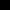
\includegraphics[scale=4]{test1}} & \fbox{
\includegraphics[scale=4]{test2}} & \fbox{
\includegraphics[scale=4]{test3}} & \fbox{
\includegraphics[scale=4]{test4}} & \fbox{
\includegraphics[scale=4]{test5}} & \fbox{
\includegraphics[scale=10]{test6}} \\[.2cm] 
PO: & \fbox{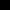
\includegraphics[scale=4]{test1_2}} & \fbox{
\includegraphics[scale=4]{test2_2}} & \fbox{
\includegraphics[scale=4]{test3_2}} & \fbox{
\includegraphics[scale=4]{test4_2}} & \fbox{
\includegraphics[scale=4]{test5_2}} & \fbox{
\includegraphics[scale=10]{test6_2}}
\end{tabular}
\end{table}

\begin{table}[H]
\caption{Porównanie plików graficznych przed i po kompresji (pomniejszone):}
\centering
\begin{tabular}{c l l l l l l}
PLIK: &test8.bmp&test9.bmp&test10.bmp&test11.bmp&test12.bmp&test13.bmp\\
PRZED & \fbox{
\includegraphics[width=.1\textwidth]{test8}} & \fbox{
\includegraphics[width=.1\textwidth]{test9}} & \fbox{
\includegraphics[width=.1\textwidth]{test10}} & \fbox{
\includegraphics[width=.1\textwidth]{test11}} & \fbox{
\includegraphics[width=.1\textwidth]{test12}} & \fbox{
\includegraphics[width=.1\textwidth]{test13}} \\[.2cm] 
PO & \fbox{
\includegraphics[width=.1\textwidth]{test8_2}} & \fbox{
\includegraphics[width=.1\textwidth]{test9_2}} & \fbox{
\includegraphics[width=.1\textwidth]{test10_2}} & \fbox{
\includegraphics[width=.1\textwidth]{test11_2}} & \fbox{
\includegraphics[width=.1\textwidth]{test12_2}} & \fbox{
\includegraphics[width=.1\textwidth]{test13_2}}
\end{tabular}
\end{table}

Porównania bajtowe wykonano programem vbindiff\cite{diff}.
\begin{figure}[H]
	\caption{Porównanie różnic dwóch tablic bajtowych przed kompresją i po dekompresji.}
	\centering
	\begin{minipage}{0.45\textwidth}
		\centering
		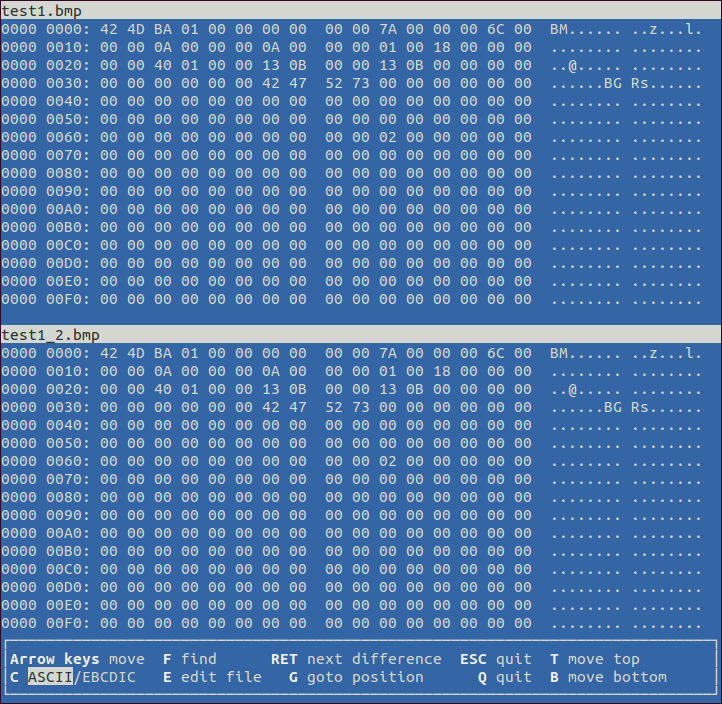
\includegraphics[scale=.3]{test1_beg}
	\end{minipage}\hfill
	\begin{minipage}{0.45\textwidth}
		\centering
		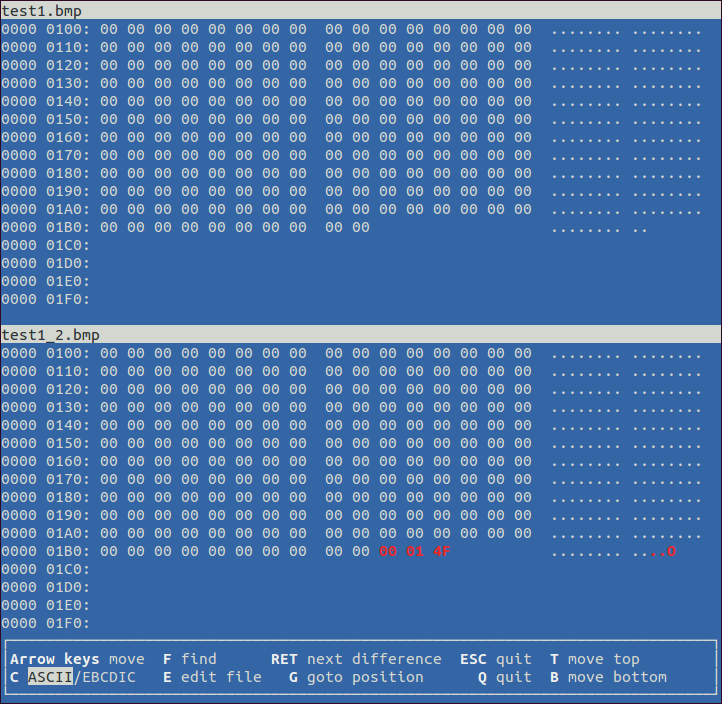
\includegraphics[scale=.3]{test1_end}
	\end{minipage}
\end{figure}

\begin{figure}[H]
	\caption{Porównanie różnic dwóch tablic bajtowych przed kompresją i po dekompresji.}
	\centering
	\begin{minipage}{0.45\textwidth}
		\centering
		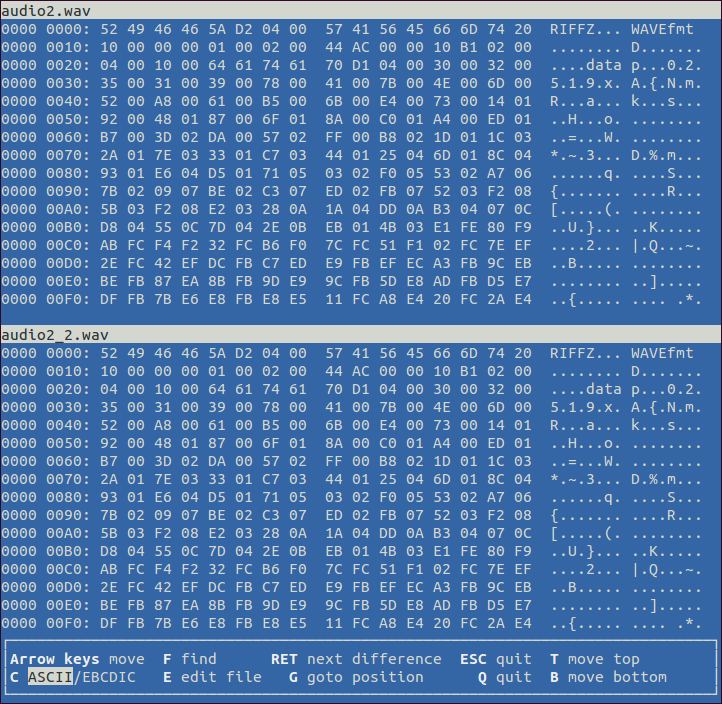
\includegraphics[scale=.3]{audio2_beg}
	\end{minipage}\hfill
	\begin{minipage}{0.45\textwidth}
		\centering
		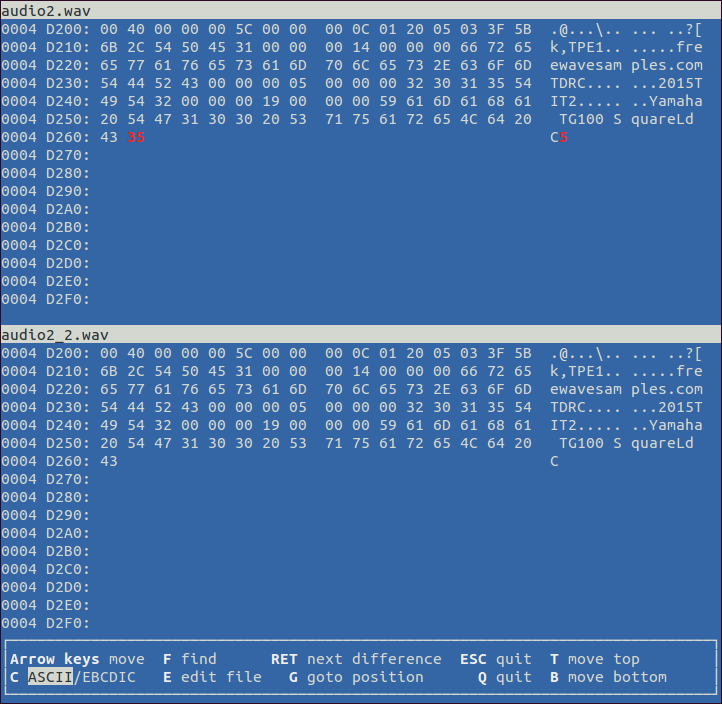
\includegraphics[scale=.3]{audio2_end}
	\end{minipage}
\end{figure}

\begin{figure}[H]
	\caption{Porównanie różnic dwóch tablic bajtowych przed kompresją i po dekompresji.}
	\centering
	\begin{minipage}{0.45\textwidth}
		\centering
		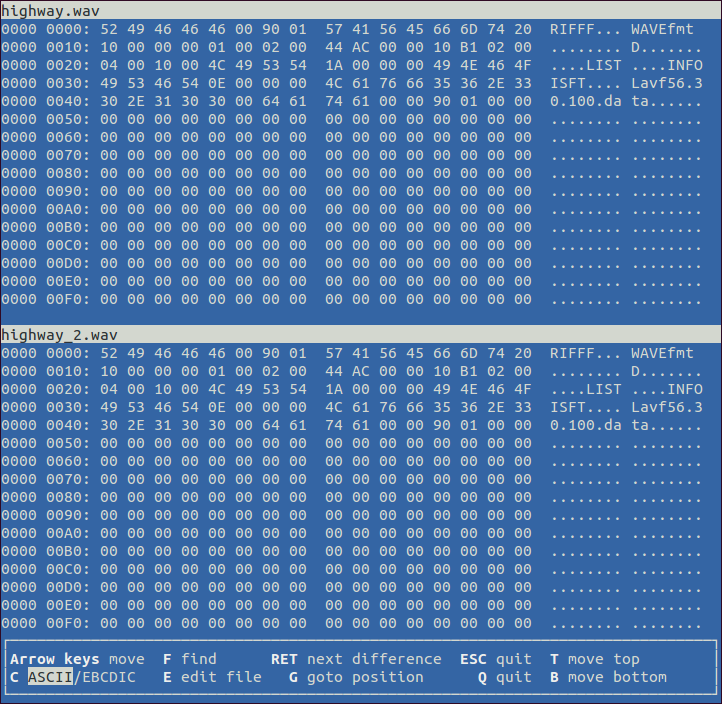
\includegraphics[scale=.3]{highway_beg}
	\end{minipage}\hfill
	\begin{minipage}{0.45\textwidth}
		\centering
		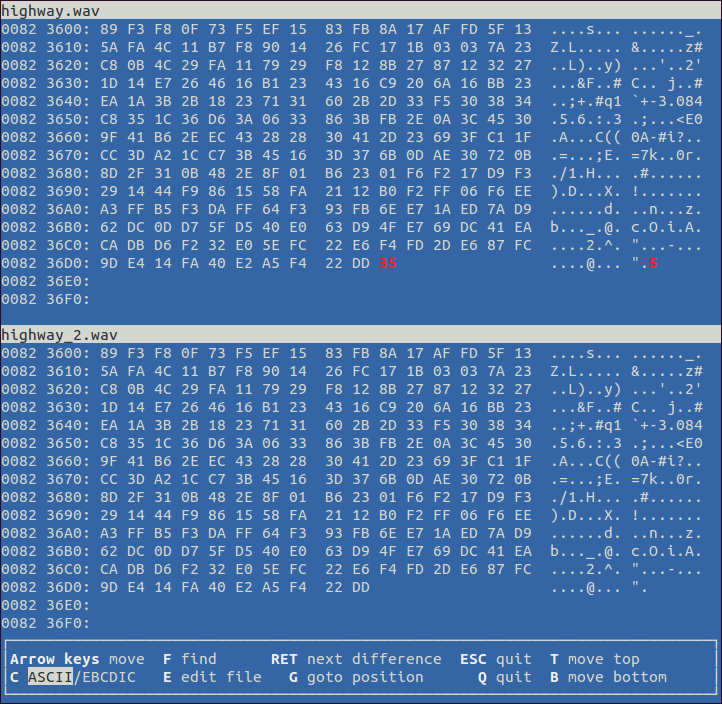
\includegraphics[scale=.3]{highway_end}
	\end{minipage}
\end{figure}

\section{Wnioski}
Algorytm \textbf{Run-Length Encoding} doskonale się sprawdza do kompresji plików graficznych monochromatycznych (jedno kolorowych) - kompresuje pliki na poziomie $20-50 \%$. Przy bardziej złożonych - bardziej kolorowych - plikach graficznych kompresja spada do poziomu $80-99\%$. Pliki dźwiękowe, z racji swojej zawiłości również nie są podatne na kompresję tym algorytmem.

Algorytm jest prosty w implementacji i obsłudze oraz dla niektórych plików może dać ,,zachwycające'' rezultaty - kompresja na poziomie tysięcznych części pliku wejściowego. Jednakże nie gwarantuje on ,,oszczędności'' miejsca - kompresji.

W procesie kompresji / dekompresji nie powstały żadne znaczące błędy. ,,Przeinaczenia'' bajtowe powstałe wskutek ,,wypełnienia'' bajtami z dekompresowanych plików nie wpływają na obiekt końcowy.\newline
Niewielkie uszkodzenia plików powstałe podczas testowania wystąpiły na skutek przeciążenia systemu innymi zadaniami.

\addcontentsline{toc}{section}{Literatura}  %dodanie znacznika "Literatura" do spisu treści
\begin{thebibliography}{1}
	\bibitem{latex} Kurs \LaTeX w $\pi^e$ minut \url{http://www.fuw.edu.pl/~kostecki/kurs_latexa.pdf}.
	\bibitem{program} Program Texmaker 4.5 \url{http://www.xm1math.net/texmaker/}.
	\bibitem{sharelatex} ShareLaTeX online LaTeX editor \url{https://www.sharelatex.com/}.	
	\bibitem{qt} Qt Creator – wieloplatformowe środowisko programistyczne \url{http://www.qt.io/}.
	\bibitem{gcc} GCC, the GNU Compiler Collection \url{https://gcc.gnu.org/}.
	\bibitem{git} Git rozproszony system kontroli wersji \url{http://git-scm.com/}.
	\bibitem{github} GitHub Web-based Git repository \url{https://github.com/}.
	\bibitem{golomb} Run-length encodings - S. W. Golomb (1966); IEEE Trans Info Theory 12(3):399 \url{http://urchin.earth.li/~twic/Golombs_Original_Paper/}.
	\bibitem{book} Variable-length codes for data compression / David Salomon, London : Springer, 2007.
	\bibitem{ikony} The largest database of free vector icons - flaticon \url{http://www.flaticon.com/}.
	\bibitem{nuty} Sample WAV files \url{http://download.wavetlan.com/SVV/Media/HTTP/http-wav.htm}.
	\bibitem{diff} vbindiff - hexadecimal file display and comparison \url{http://manpages.ubuntu.com/manpages/hardy/man1/vbindiff.1.html}.
\end{thebibliography}

	\blfootnote{Dokument wykonany w \LaTeX \cite{latex} \\ w programie Texmaker 4.5 \cite{program}}	
\end{document}
%\begin{lstlisting}[language=C++, caption={}]
%\end{lstlisting}
